\section{کاهش رزولوشن بدون فیلتر و بررسی روش‌های درونیابی}

در این بخش، قصد داریم تصاویر را بدون اعمال هیچ‌گونه فیلتر پایین‌گذر (Anti-aliasing) و تنها با حذف مستقیم پیکسل‌ها، با نرخ‌های ۴ و ۱۶ کوچک کنیم. سپس برای مشاهده‌ی دقیق‌تر آثار مخرب این کار و بررسی پدیده الیاسینگ، تصاویر کوچک‌شده را با دو روش «نزدیک‌ترین همسایه» و «دوخطی» به ابعاد اولیه بازمی‌گردانیم تا تفاوت الگوریتم‌های درونیابی (\lr{Interpolation}) را بررسی کنیم.

\subsection*{۱. آماده‌سازی و دریافت ابعاد تصویر}
در ابتدای کار، پوشه خروجی را ایجاد کرده و ابعاد تصویر اصلی را ذخیره می‌کنیم:

\begin{codebox}[\lr{Setup and Dimensions}]
\begin{lstlisting}[language=Python]
output_dir_2 = "./Output_Images/Part_2"
os.makedirs(output_dir_2, exist_ok=True)

rates = [4, 16]

for title, img in images_8bit.items():
    original_height, original_width = img.shape
    
    for r in rates:
\end{lstlisting}
\end{codebox}

ذخیره کردن ابعاد تصویر اصلی (\lr{\texttt{original\_height}} و \lr{\texttt{original\_width}}) بسیار مهم است؛ زیرا در مراحل بعدی که تصویر را کوچک می‌کنیم، برای بازگرداندن آن به سایز اولیه‌اش (جهت مقایسه چشمی) به این ابعاد نیاز خواهیم داشت.

\subsection*{۲. کاهش ابعاد (Downsampling) خام}
در این مرحله، عمل نمونه‌برداری کاهشی را بدون هیچ فیلتری انجام می‌دهیم:

\begin{codebox}[\lr{Sub-sampling}]
\begin{lstlisting}[language=Python]
        # Downsampling (کاهش ابعاد بدون فیلتر)
        downsampled_img = img[::r, ::r]
\end{lstlisting}
\end{codebox}

دستور \lr{\texttt{img[::r, ::r]}} از قابلیت \lr{Slicing} در آرایه‌های نامپای استفاده می‌کند. این خط کد به زبان ساده می‌گوید: «سطرها و ستون‌ها را از ابتدا تا انتها طی کن، اما گام‌هایت را $r$تایی بردار». این یعنی از هر $r$ پیکسل، تنها پیکسل اول حفظ شده و بقیه حذف می‌شوند. از آنجا که فرکانس‌های بالا پیش از این کار فیلتر نشده‌اند، در همین خط پدیده مخرب الیاسینگ رخ می‌دهد.

\subsection*{۳. بازسازی با روش نزدیک‌ترین همسایه \lr{(NearestNeighbor)}}
حالا تصویر کوچک‌شده را با ساده‌ترین روش درونیابی به سایز اصلی برمی‌گردانیم:

\begin{codebox}[\lr{Nearest Neighbor Interpolation}]
\begin{lstlisting}[language=Python]
        # Upsampling (روش نزدیک‌ترین همسایه)
        upsampled_nn = cv2.resize(downsampled_img, 
                                  (original_width, original_height), 
                                  interpolation=cv2.INTER_NEAREST)
\end{lstlisting}
\end{codebox}

الگوریتم \lr{\texttt{INTER\_NEAREST}} برای تولید پیکسل‌های جدیدی که در فرآیند کوچک‌سازی از دست رفته‌اند، هیچ محاسبه‌ی ریاضی پیچیده‌ای انجام نمی‌دهد؛ بلکه صرفاً مقدار نزدیک‌ترین پیکسلِ موجود را کپی می‌کند. این کار بسیار سریع است اما لبه‌هایی به‌شدت دندانه‌دار و تصاویری بلوکی (شطرنجی) تولید می‌کند.

\subsection*{۴. بازسازی با روش دوخطی (Bilinear)}
در قدم بعدی، بازسازی را با روشی پیشرفته‌تر انجام می‌دهیم:

\begin{codebox}[\lr{Bilinear Interpolation}]
\begin{lstlisting}[language=Python]
        # Upsampling (روش دوخطی)
        upsampled_bl = cv2.resize(downsampled_img, 
                                  (original_width, original_height), 
                                  interpolation=cv2.INTER_LINEAR)
\end{lstlisting}
\end{codebox}

در الگوریتم \lr{\texttt{INTER\_LINEAR}}، برای تعیین شدت روشنایی یک پیکسل جدید، میانگین وزن‌دار ۴ پیکسل مجاور آن محاسبه می‌شود. این روش باعث نرم‌تر شدن لبه‌ها و کاهش حالت شطرنجی می‌شود، اما در عین حال تصویر را تا حدودی تار (\lr{Blur}) می‌کند.

این نام‌گذاری منظم (شامل نام تصویر، نرخ کاهش و روش بازسازی) به ما کمک می‌کند تا در زمان تهیه گزارش، تصاویر را به راحتی فراخوانی و مقایسه کنیم.

\subsection*{نمایش خروجی‌ها (نمونه: تصویر \lr{Grid})}
به دلیل وجود الگوهای تکرارشونده و لبه‌های تیز در تصویر \lr{Grid}، پدیده الیاسینگ در این تصویر با وضوح بیشتری قابل مشاهده است. در شکل زیر، نتایج بازسازی این تصویر را مشاهده می‌کنید:

\begin{figure}[h!]
    \centering
    \begin{subfigure}{0.48\textwidth}
        \centering
        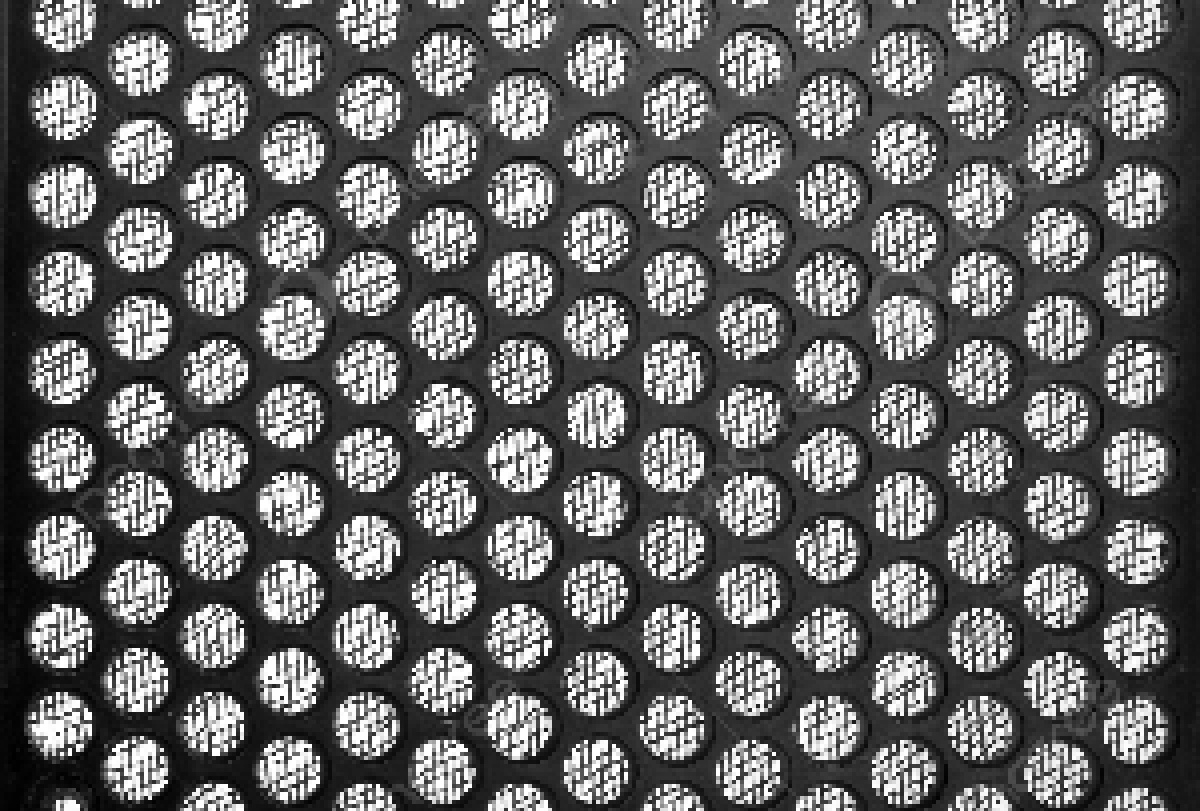
\includegraphics[width=\textwidth]{images/2_Rate4_Nearest.jpg}
        \caption{نرخ ۴ - درونیابی نزدیک‌ترین همسایه}
    \end{subfigure}
    \hfill
    \begin{subfigure}{0.48\textwidth}
        \centering
        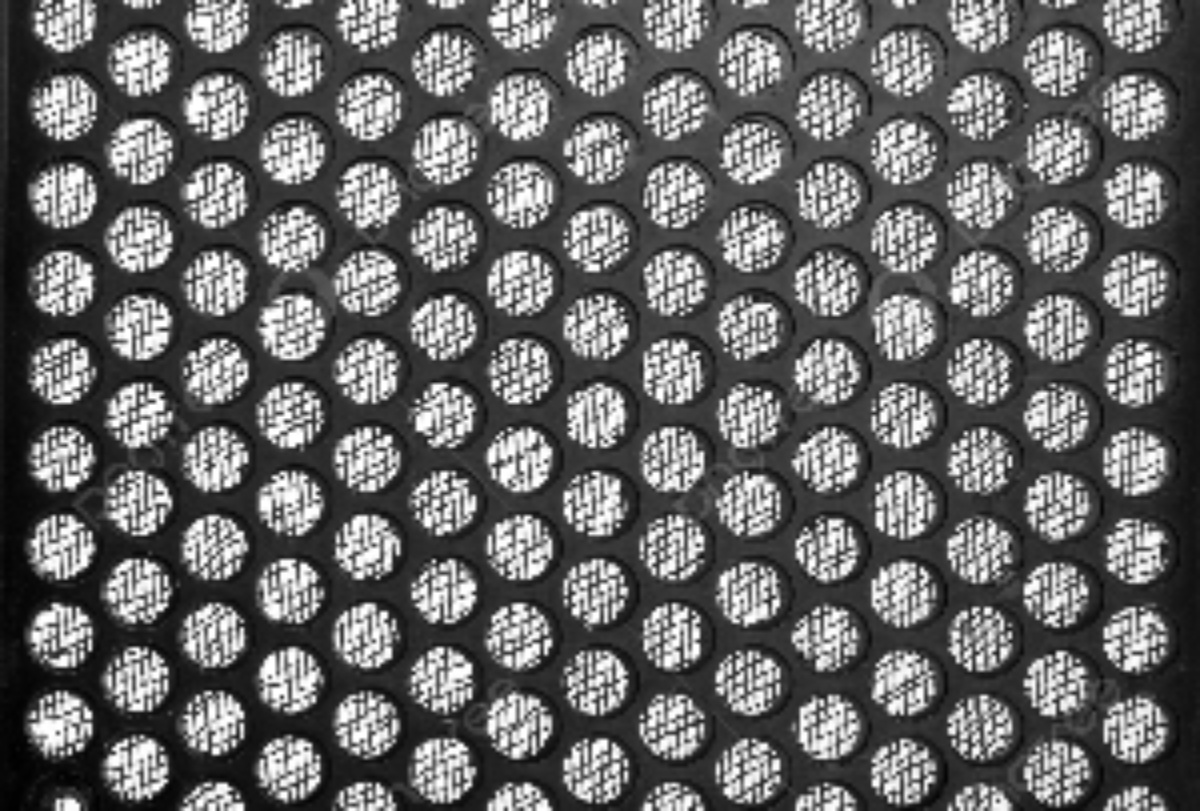
\includegraphics[width=\textwidth]{images/2_Rate4_Bilinear.jpg}
        \caption{نرخ ۴ - درونیابی دوخطی}
    \end{subfigure}
    
    \vspace{0.4cm}
    
    \begin{subfigure}{0.48\textwidth}
        \centering
        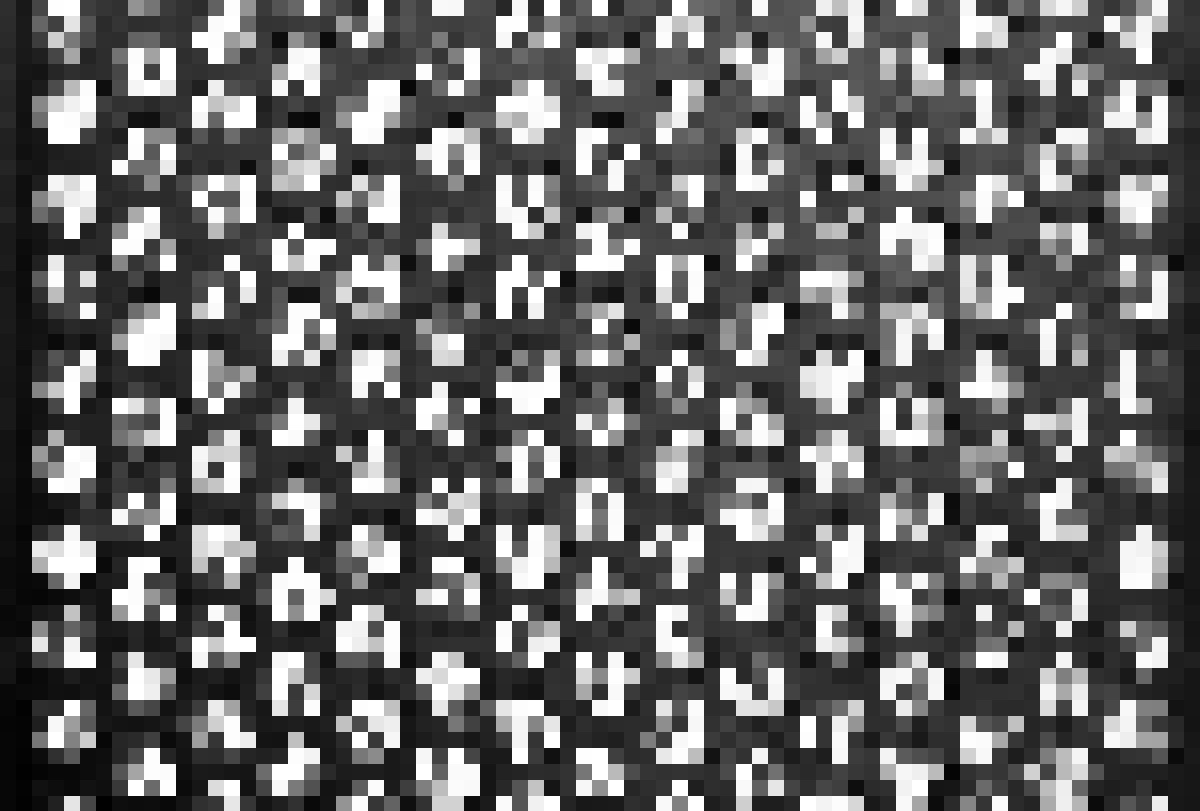
\includegraphics[width=\textwidth]{images/2_Rate16_Nearest.jpg}
        \caption{نرخ ۱۶ - درونیابی نزدیک‌ترین همسایه}
    \end{subfigure}
    \hfill
    \begin{subfigure}{0.48\textwidth}
        \centering
        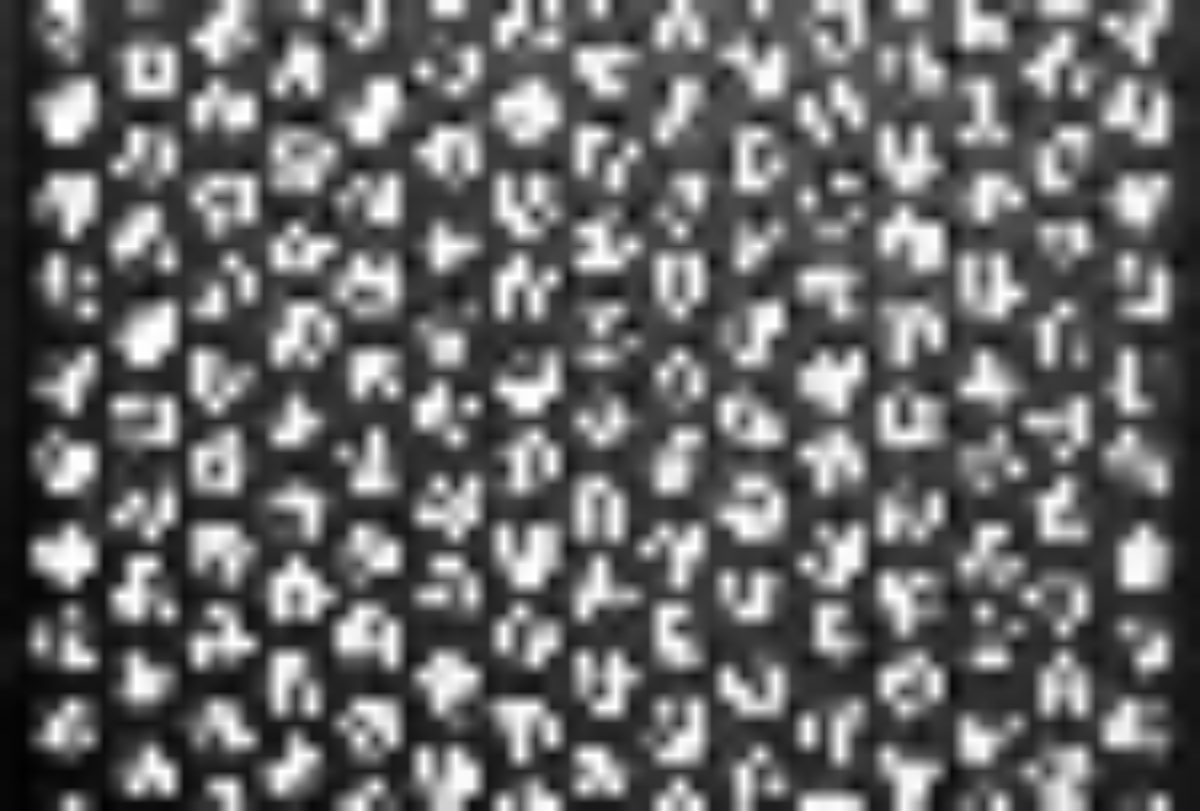
\includegraphics[width=\textwidth]{images/2_Rate16_Bilinear.jpg}
        \caption{نرخ ۱۶ - درونیابی دوخطی}
    \end{subfigure}
    \caption{مقایسه تأثیر نرخ‌های مختلف کاهش رزولوشن و روش‌های درونیابی بر پدیده \lr{Aliasing} در تصویر \lr{Grid}}
    \label{fig:part2_grid_comparison}
\end{figure}

\newpage
\subsection*{تحلیل خروجی‌ها و بررسی پدیده \lr{Aliasing}}
با دقت در تصاویر تولید شده (شکل \ref{fig:part2_grid_comparison})، می‌توان به نتایج مهم زیر دست یافت:

\begin{itemize}
    \item \textbf{ایجاد \lr{Moiré Pattern}:} در تصاویر مربوط به نرخ ۴، به وضوح الگوهای جدیدی (خطوط مورب و بافت‌های کاذب) در داخل دایره‌های شبکه ایجاد شده‌اند که در تصویر اصلی وجود نداشتند. این الگوهای مزاحم (\lr{Moiré Pattern})، دقیقاً همان پدیده الیاسینگ هستند که به دلیل نمونه‌برداری خام و بدون فیلتر به وجود آمده‌اند.
    
    \item \textbf{تأثیر روش‌های درونیابی در مهار الیاسینگ:} روش \lr{Nearest} مرزهای بسیار دندانه‌دار تولید کرده است. در مقابل، روش \lr{Bilinear} مرزها را نرم‌تر کرده است. اما نکته کلیدی اینجاست: روش دوخطی الگوهای مخرب الیاسینگ را از بین نبرده است؛ زیرا این اطلاعات کاذب در مرحله‌ی \lr{Slicing} وارد تصویر شده‌اند و درونیابی دوخطی تنها این اطلاعات غلط را تارتر کرده است.
    
    \item \textbf{فاجعه‌ی نرخ ۱۶:} در نرخ ۱۶، کاهش رزولوشن به حدی شدید است که تقریباً تمام فرکانس‌های پایه‌ی تصویر از دست می‌رود. در روش \lr{Nearest} تصویر به مجموعه‌ای از مربع‌های تصادفی تبدیل شده و در روش \lr{Bilinear} این مربع‌ها به شکل لکه‌هایی تار (\lr{Blobs}) درآمده‌اند. بازسازی ساختار شبکه‌ای در این نرخ عملاً غیرممکن است.
\end{itemize}